\documentclass[14pt]{article}

\usepackage[margin=20mm]{geometry}
\geometry{
        a4paper,
        total={165mm,247mm},
        top=30mm,
        bottom=20mm
%       evenmargin=25mm,
%       oddsidemargine=20mm
%       left=20mm
}


\usepackage[utf8]{inputenc}
\usepackage[russian]{babel}
\usepackage[usenames]{color}
\usepackage{amsmath}
\usepackage{amssymb}        % for \varnothing

\usepackage{tikz}
\usepackage{siunitx}
\usepackage[american,cuteinductors,smartlabels]{circuitikz}

\usepackage{pdfpages}

\usepackage{booktabs}

% для физики
\usetikzlibrary{arrows,shapes,positioning}
\usetikzlibrary{decorations.markings,decorations.pathmorphing,
decorations.pathreplacing}
\usetikzlibrary{calc,patterns,shapes.geometric}

\usepackage{xcolor}
\usepackage{hyperref}

\definecolor{linkcolor}{HTML}{799B03} % цвет ссылок
\definecolor{urlcolor}{HTML}{799B03} % цвет гиперссылок

\hypersetup{pdfstartview=FitH,  linkcolor=linkcolor,urlcolor=urlcolor, colorlinks=true}

\definecolor{AleeGreen}{rgb}{0.4,0.8,0.4}

\usepackage{lettrine}
%\usepackage{amsmath}
\usepackage{amsfonts}
\usepackage{dsfont}


\tikzset{
        position label/.style={
                below = 3pt,
                text height = 1.5ex,
                text depth = 1ex
        },
        brace/.style={
                decoration={brace, mirror},
                decorate
        }
}

\usepackage{multirow}
\usepackage{multicol}

\begin{document}

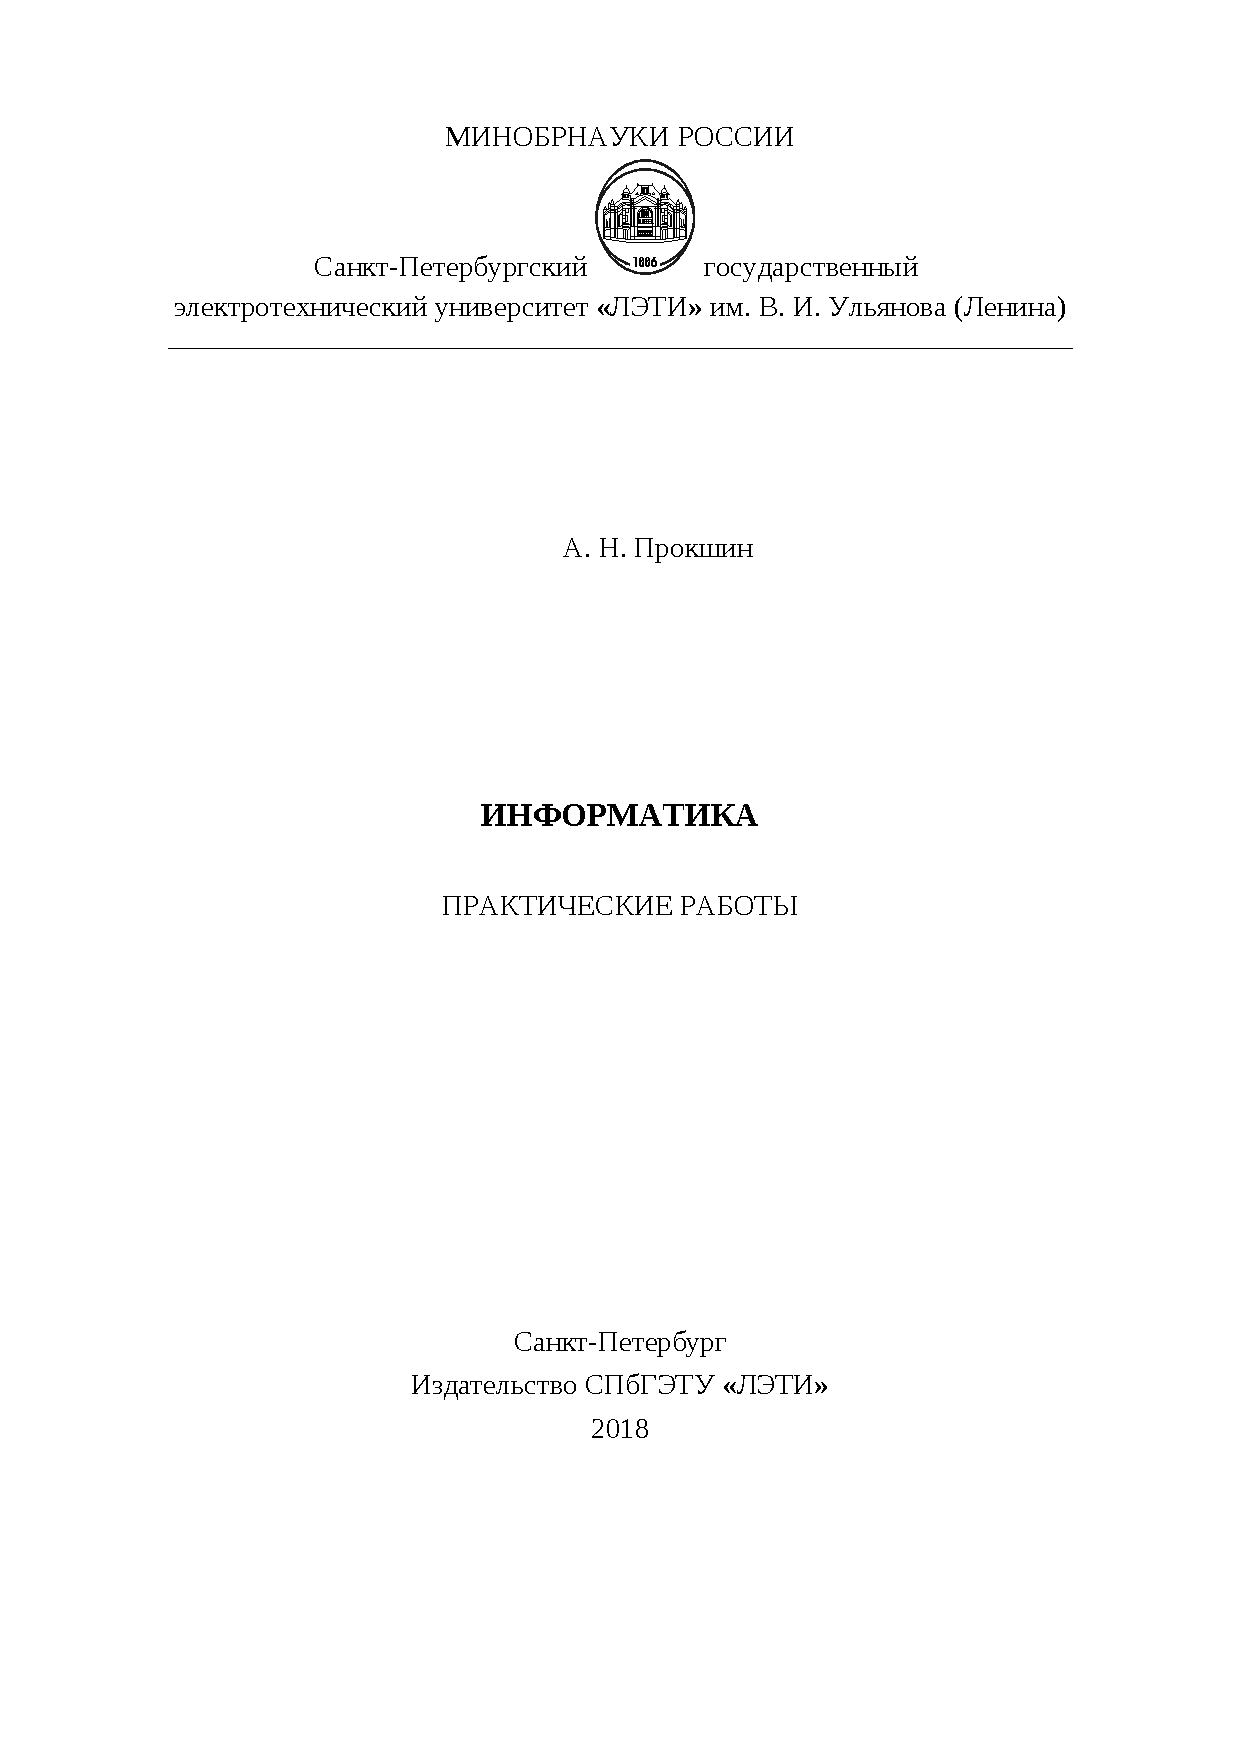
\includepdf[pages=-]{Informatika_praktika_title}

\begin{abstract}
Излагаются основы оформления документации в издательской системе Латех. Ряд практических работ раскрывает принципы построения аппаратной части компьютеров и компьютерных графических систем.
Другая часть практических работ предназначена для формирования навыков создания электронных документов электротехнического и общенаучного направления.

Практические работы по дисциплине «Информатика» предназначены для бакалавров по направлению подготовки 13.03.02 «Электроэнергетика и электротехника» профилю «Электропривод и автоматика».
\end{abstract}

\newpage
\tableofcontents

\newpage

\subsection{Введение}

\LaTeX широко используется для оформления научной и технической литературы, статей. На вебсайтах при оформлении формул
используется \LaTeX. Примеры сайтов -- wikipedia, openedu.ru
Также оформление формул в виде \LaTeX имеется в GeoGebra

Документ в \TeX или \LaTeX представляет собой текстовый файл с расширением {\bf.tex}, который можно открыть любым текстовым редактором.
Если не обращать внимание на команды, то текст можно свободно читать.
Документы можно оформлять в любой кодировке, однако стандартом сейчас является кодировка utf-8.

Минимальный документ выглядит так:

\begin{verbatim}
\documentclass{minimal}
\usepackage[utf8]{inputenc}
\usepackage[russian]{babel}

\begin{document}
Приведём выражение для $sin(\alpha + \beta)$ синуса суммы:

$$ 
sin(\alpha + \beta)  = cos(\alpha) \cdot sin(\beta) + sin(\alpha)\cdot cos(\beta)
$$

\end{document}
\end{verbatim}

Простейшие правила:
\begin{itemize}
	\item любое количество пробелов, символов табуляций и единичный символ перевода строки считается за один пробел;
	\item абзацы отделяются друг от друга пустой строкой;
	\item в тексте могут встречаться команды, которые начинаются с символа $\backslash$  -- backslash;
	\item команды могут снабжаться параметрами в фигурных скобках \{\}, и модификаторами [ ]; 
	\item для математических формул используется математическая мода. В тексте математическая мода выделяется
		с двух сторон знаком \$, выключнная математическая формула выделяется с обеих сторон удвоенными знаками \$\$;
	      \item комментарий в строке начинается с символа \%.
        \item дефис -- это один знак ``-'', для тире лучше использовать двойной знак ``-'' или тройной.
\end{itemize}

Нумерация формул задается внутри окружения {\bf equation}:

\begin{verbatim}
\begin{equation}
\cos(\alpha + \beta)  = cos(\alpha) \cdot \cos(\beta) - sin(\alpha)\cdot \sin(\beta)
\end{equation}
\label{equation.first_equation}
\end{verbatim}

Выключная формула с нумерацией выглядит так:
\begin{equation}                                                                                                                                                         \cos(\alpha + \beta)  = cos(\alpha) \cdot \cos(\beta) - sin(\alpha)\cdot \sin(\beta)                                                                                     \end{equation}                                                                                                                                                            \label{equation.first_equation}  

На формулу, и на любое окружение, отмеченное командой {\bf $\backslash$label}\{имя метки\} можно сослаться в любом месте  (\ref{equation.first_equation}) командой
{\bf $\backslash$ref}\{имя метки\} 

% https://www.ibm.com/developerworks/ru/library/latex_tutorial_01/

На первой строке загружается класс документа {\bf minimal}. В следующих строках загружаются стилевые файлы, необходимые для руссификации документа.
\begin{itemize}
	\item[]{\color{red}{inputenc}} -- для выбора кодировки текстового файла; 
	\item[]{\color{red}{babel}} --  пакет для локализаци.
\end{itemize}

Сам текст документа набирается внутри окружения document, которое начинается с команды {\bf$\backslash$begin\{document\}} и заканчивается конструкцией {\bf$\backslash$end\{document\}}. 

Чтобы скомпилировать исходный текст и получить документ в формате pdf следует воспользоваться командой {\bf pdflatex} и затем увидеть полученный результат командой {\bf evince}:
\begin{verbatim}
pdflatex <ваш файл>.tex
evince <ваш файл>.pdf
\end{verbatim}

В OS Linux команда {\bf pdflatex} доступна при установке программ из набора {\bf texlive},
в OS windows распространенный набор {\bf MikTeX}, в MacOS -- MacTex.
Можно также выбрать специализированный \LaTeX-редактор, например, Texmaker или TeXstudio. 

Доступны онлайн-сервисы \href{https://www.sharelatex.com}{https://www.sharelatex.com} и \href{https://www.overleaf.com}{https://www.overleaf.com}. 


В математической моде нижние и верхние индексы задаются после символов $\_$ и $\hat{}$, которые действуют только на один последующий символ. 
Чтобы поместить несколько символов в индекс, нужно поместить их в фигурные скобки. Фигурные скобки ограничивают блок. 


Выражение
\begin{minipage}{1in}
\begin{verbatim}
$A^{ij}_{bk}$
\end{verbatim}
\end{minipage} 
даст 
\begin{minipage}{1in}	
\begin{circuitikz}
	\draw (0,0) rectangle (2,0.6)
	(1,0.3) node {$A^{ij}_{bk}$}; 
\end{circuitikz}
\end{minipage}

В случаях со знаками сумм, интегралов, пределов нужно поместить индексы непосредственно над и под знаками

\begin{minipage}{2.5in}
\begin{verbatim}
\int\limits_{-\infty}^{+\infty}
\end{verbatim}
\end{minipage}
\begin{minipage}{1in}
\begin{circuitikz}
        \draw (0,0) rectangle (2,0.9)
	(1,0.45) node {$\int\limits_{-\infty}^\infty$};
\end{circuitikz}
\end{minipage}


\begin{minipage}{2.5in}
\begin{verbatim}
\sum\limits_{k=0}^{10} A_k
\end{verbatim}
\end{minipage}
$
\sum\limits_{k=0}^{10} A_k
$

% http://www.intuit.ru/studies/courses/1137/137/lecture/3839?page=2
% https://tex.stackexchange.com/questions/20575/attractive-boxed-equations  -- boxed
%https://repetitors.info/otvet/?t=6514
{\color{red}
  \boxed{ % from \usepackage{amsmath}
    {\color{black}
      \int\limits_a^bf(t)\,dt = \Phi(b) - \Phi(a) \stackrel{\text{def}}{=} \Bigl.\Phi(t)\Bigl|_{t=a}^{t=b}
    }
  }
}

Греческие буквы выглядят как $\backslash$ + английское название буквы:

\begin{tabular}{|llll|} \hline % or any other width
%  \rule{0pt}{5ex}% for more vertical space
$\alpha$ & \begin{minipage}{1in}\begin{verbatim} \alpha \end{verbatim}\end{minipage} & &\\
$\beta$ & \begin{minipage}{1in}\begin{verbatim} \beta \end{verbatim}\end{minipage} & &\\
$\gamma$ & \begin{minipage}{1in}\begin{verbatim} \gamma \end{verbatim}\end{minipage} & $\Gamma$ & \begin{minipage}{1in}\begin{verbatim} \Gamma \end{verbatim}\end{minipage}\\
$\delta$ & \begin{minipage}{1in}\begin{verbatim} \delta \end{verbatim}\end{minipage} & $\Delta$ & \begin{minipage}{1in}\begin{verbatim} \Delta \end{verbatim}\end{minipage}\\ 
$\zeta$ & \begin{minipage}{1in}\begin{verbatim} \zeta \end{verbatim}\end{minipage}   &&\\
$\xi$ & \begin{minipage}{1in}\begin{verbatim} \xi \end{verbatim}\end{minipage} & &\\
$\phi$ & \begin{minipage}{1in}\begin{verbatim} \phi \end{verbatim}\end{minipage} & &\\
$\varphi$ & \begin{minipage}{1in}\begin{verbatim} \varphi \end{verbatim}\end{minipage} & &\\

$\omega$ & \begin{minipage}{1in}\begin{verbatim} \omega \end{verbatim}\end{minipage} & $\Omega$ & \begin{minipage}{1in}\begin{verbatim} \Omega \end{verbatim}\end{minipage}\\\hline
\end{tabular}
\\

%https://tex.stackexchange.com/questions/40774/placing-text-and-equations-inside-a-box

Таблицы -- не самое сильное место \LaTeX :

\begin{verbatim}
\begin{tabular}{|c|c|c|c|} \hline
  1 & 2 & 3 & 4 \\
  \hline
  5 & 6 & 7 & 8 \\
  \hline
\end{tabular}  
\end{verbatim}

\begin{tabular}{|c|c|c|c|} \hline
  1 & 2 & 3 & 4 \\
  \hline
  5 & 6 & 7 & 8 \\
  \hline
\end{tabular}

Дать название тaблице (\ref{table.sample}) и метку для ссылки можно в окружениии {\bf table}

\begin{verbatim}
\begin{table}[ht]
  \centering
\begin{tabular}{|c|c|c|c|} \hline                                                                                                                      	       	
   1 & 2 & 3 & 4 \\
  \hline
  5 & 6 & 7 & 8 \\
  \hline
\end{tabular}
\label{table.sample}
\caption{Пример таблицы}
\end{table}
\end{verbatim}

\begin{table}[ht]
  \centering
\begin{tabular}{|c|c|c|c|} \hline                                                                                                                                        
   1 & 2 & 3 & 4 \\
  \hline
  5 & 6 & 7 & 8 \\                                                                                                                                                       
  \hline                                                                                                                                                                 
\end{tabular}
\label{table.sample}
\caption{Пример таблицы}
\end{table}

Можно оформить таблицу в книжном стиле. Для этого нужно добавить пакет {\bf $\backslash$usepackage\{booktabs\}}

\begin{verbatim}
\begin{tabular}{p{6pt}|p{6pt}|p{0.2\linewidth}}
  \toprule
  &\multicolumn{2}{c}{test}\\
  \cmidrule{2-3}
  \rotatebox{90}{\rlap{\small прак.}} &1&2\\
  \midrule
  4&5&6\\
\bottomrule
\end{tabular}
\end{verbatim}

\begin{tabular}{p{6pt}|p{6pt}|p{0.2\linewidth}}
  \toprule
  &\multicolumn{2}{c}{test}\\
  \cmidrule{2-3}
  \rotatebox{90}{\rlap{\small прак.}} &1&2\\
  \midrule
  4&5&6\\
\bottomrule
\end{tabular}
\\

Оформление систем и совокупностей уравнений и неравенств
\begin{verbatim}
$$
\left\{
\begin{array}{lll}
  x^2 - y  & \ge & 0 \\
  3x + 2y & \le & 3 \\
\end{array}
\right.
$$
\end{verbatim}

$$
\left\{\begin{array}{lll}
  x^2 - y  & \geq & 0 \\
  3x + 2y & \leq & 3 \\
\end{array}
\right.
$$

% http://oeis.org/wiki/List_of_LaTeX_mathematical_symbols
% http://w2.syronex.com/jmr/tex/texsym.old.html
\begin{table}[ht]
\caption{Краткий список символов в математической моде}
\begin{tabular}{ll|ll|ll|ll}
\toprule  
  \multicolumn{2}{c|}{relational} & \multicolumn{2}{c|}{logic} & \multicolumn{2}{c|}{set} & \multicolumn{2}{c}{miscellaneous}\\
symbol & command & symbol & command & symbol & command & symbol & command\\
  \midrule
  $\equiv$ & $\backslash$equiv   & $\bullet$ & $\backslash$bullet                       & $\cap$ & $\backslash$cap               & $\prime$ & $\backslash$prime \\
  $\approx$ & $\backslash$approx & $\neg$ & $\backslash$neg                             & $\cup$ & $\backslash$cup               & $\infty$ & $\backslash$infty \\
  $\propto$ & $\backslash$propto & $\wedge,\land$ & $\backslash$wedge,$\backslash$land  & $\supset$ & $\backslash$supset         & $\circ$  & $\backslash$circ \\
  $\simeq$ & $\backslash$simset  & $\vee,\lor$  & $\backslash$vee,$\backslash$lor       & $\subset$ & $\backslash$subset         & $\angle$ & $\backslash$angle \\
  $\sim$   & $\backslash$sim     & $\oplus$ & $\backslash$oplus                         & $\varnothing$ & $\backslash$varnothing & $\triangle$ & $\backslash$triangle \\
  $\neq$   & $\backslash$neq     & $\Rightarrow$ & $\backslash$Rightarrow               & $\in$ & $\backslash$in                 & $\cong$ & $\backslash$cong \\
  $\geq$   & $\backslash$geq     & $\Leftrightarrow$ & $\backslash$Leftrightarrow       & $\notin$ & $\backslash$notin           & $\pm$   & $\backslash$pm \\
  $\gg$    & $\backslash$gg      & $\exists$ & $\backslash$exists                       & $\ni$ & $\backslash$ni                 & $\mp$   & $\backslash$mp \\
  $\ll$    & $\backslash$ll      & $\forall$ & $\backslash$forall                       & $\cdot$ & $\backslash$cdot             & $\times$ & $\backslash$times \\
  \bottomrule
\end{tabular}
\end{table}

Представления дробей:

\begin{tabular}{ccc}
\begin{minipage}{2in}
\begin{verbatim}
$$
\frac{1}{1+n^2}
$$
\end{verbatim}
\end{minipage}
& $\rightarrow$ &
$
\boxed{\frac{1}{1+n^2}}
$
\end{tabular}

Подчеркивания:

\begin{tabular}{ccc}
  \begin{minipage}{3in}
\begin{verbatim}    
$$
  \underbrace{
    \frac{1}{1+n^2}
  }_\text{элемент последовательности}
$$
\end{verbatim}  
\end{minipage}
&$\rightarrow$ &
$
  \underbrace{
    \frac{1}{1+n^2}
  }_\text{\begin{tabular}{c}элемент\\последовательности\end{tabular}}
$
  
\end{tabular}

\subsection{Шрифты}
Размер:
tiny, scriptsize, footnotesize, small,normalsize,large,Large,LARGE, huge,Huge

\noindent {\tiny tiny} {\scriptsize scriptsize} {\footnotesize footnotesize} {\small small} {\normalsize normalsize} {\large large} {\Large Large} {\LARGE large} {\huge huge} {\Huge Huge}


\vspace{5mm}
установка размера шрифта:
\begin{verbatim}
{\scriptsize scriptsize} {\footnotesize footnotesize} {\small small} 
\end{verbatim}

\begin{table}[ht]
  \caption{Семейства шрифтов}
  \begin{tabular}{llll}
    семейство & команда & команда переключения & полученный результат\\
    \midrule
    serif (roman) 	& $\backslash$textrm\{Sample Text 0123\} 	& $\backslash$rmfamily & \textrm{Sample Text 0123}\\
    sans serif 	& $\backslash$textsf\{Sample Text 0123\} 	& $\backslash$sffamily & \textsf{Sample Text 0123}\\
\!\begin{tabular}{l}\!typewriter\\\!(monospace)\end{tabular} &	$\backslash$texttt\{Sample Text 0123\} & 	$\backslash$ttfamily & \texttt{Sample Text 0123}\\
  \end{tabular}  
\end{table}  

\begin{table}[ht]
  \caption{Стили шрифтов}
  \begin{tabular}{lllll}
    стили & команда & переключение & альтернативное	& полученный результат\\
    \midrule
    medium &	$\backslash$textmd\{Sample Text 0123\} & 	$\backslash$mdseries & &  \textmd{Sample Text 0123} \\
    bold &	$\backslash$textbf\{Sample Text 0123\} &	$\backslash$bfseries & $\backslash$bf &\textbf{Sample Text 0123} \\
    upright & 	$\backslash$textup\{Sample Text 0123\} & 	$\backslash$upshape & &\textup{Sample Text 0123}\\
    italic &	$\backslash$textit\{Sample Text 0123\} &	$\backslash$itshape &$\backslash$it &\textit{Sample }{\it Text 0123}\\
    slanted & 	$\backslash$textsl\{Sample Text 0123\} &	$\backslash$slshape &$\backslash$sl &\textsl{Sample }{\sl Text 0123}\\
    small caps& $\backslash$textsc\{Sample Text 0123\} &	$\backslash$scshape &$\backslash$sc &\textsc{Sample }{\sc Text 0123}\\
  \end{tabular}
\end{table}    

\subsection{Практическая работа №1: перевод числа из одной системы счисления в другую}

$77_{10} = 1001101_2$

Алгоритм перевода десятичного числа в двоичное следующий:
Разделим исходное число на 2. Остаток от деления будет последним знаком в искомом двоичном числе.
Целую часть(неполное частное) от деления снова поделим на 2. Остаток от деления будет следующим знаком в искомом двоичном числе.
Так будем продолжать до тех пор, пока деление возможно.

Можно воспользоваться делением ``столбиком'' и соберём остатки от деления в обратном порядке:

\begin{tikzpicture}
  \draw (0.85,5.25) node {7} (1.15,5.25) node {7}
  (1.5,4.75) -- (1.5,5.5)  (1.5,5) -- (2.4,5)
  (2,5.25) node {2} (2,4.75) node {3} (2.3,4.75) node {8}
  (0.85,4.95) node{6} (0.4,5.1) node {$-$} (0.7,4.7) -- (1.0,4.7) (0.85,4.45) node {1} (1.15,4.45) node {7}
  (0.85,4.15) node {1} (1.15,4.15) node {6}
  (0.4,4.3)  node {$-$} (0.7,3.9) -- (1.3,3.9) (1.15,3.65) node {1}; \draw[red]  (1.15,3.65) circle (0.2125);
  \draw (2.65,4.25) -- (2.65, 5) (2.65, 4.5) -- (3.55, 4.5)
  (3.15,4.75) node {2} (3.15,4.25) node {1} (3.45,4.25) node {9}
  (2,4.45) node {2} (1.7,4.6) node {$-$}  (1.85,4.2) -- (2.15,4.2) (2,3.95) node {1} (2.3,3.95) node {8}
  (2,3.65) node {1} (2.3,3.65) node {8}
  (1.7,3.8) node {$-$} (1.75,3.4) -- (2.45, 3.4) (2.3,3.15) node {0}; \draw[red] (2.3,3.15) circle (0.2125);
  \draw (3.8, 3.75) -- (3.8, 4.5) (3.8,4) -- (4.4,4)
  (4.3,4.25) node {2}  (4.3,3.75) node {9}
  (3.15,3.95) node {1} (3.45,3.95) node {8}
  (2.85,4.1) node {$-$} (3,3.7) -- (3.6, 3.7) (3.45,3.4) node {1}; \draw[red] (3.45,3.4) circle (0.2125);
  \draw (4.65, 3.25) -- (4.65,4) (4.65, 3.5) -- (5.25,3.5)
  (5.15,3.75) node {2} (5.15,3.25) node {4}
  (4.3,3.45) node {8}
  (4,3.6) node {$-$} (4.15,3.2) -- (4.45,3.2) (4.3,2.95) node {1}; \draw[red] (4.3,2.95) circle (0.2125);
  \draw (5.5, 2.75) -- (5.5, 3.5) (5.5, 3) -- (6.1, 3)
  (6,3.25) node {2} (6, 2.75) node {2}
  (5.15,2.95) node {4}
  (4.85,3.1) node {$-$} (5,2.7) -- (5.3,2.7) (5.15,2.45) node {0}; \draw[red] (5.15,2.45) circle (0.2125);
  \draw (6.35,2.25) -- (6.35,3) (6.35,2.5) -- (6.95,2.5)
  (6.85, 2.75) node {2} (6.85, 2.25) node {1}; \draw[red] (6.85, 2.25) circle (0.2125);
  \draw (6, 2.45) node {2}
  (5.7, 2.6)  node {$-$} (5.85,2.2) -- (6.15,2.2) (6,1.95) node {0}; \draw[red] (6,1.95) circle (0.2125); 
\end{tikzpicture}

Предлагаемый отчет вывыглядит примерно так:
$$
%\lceil \frac{77}{2} \rceil = 38,
\lfloor \frac{77}{2} \rfloor = 38,\quad  77\ mod\ 2 = 1 ; 
$$
$$
\lfloor \frac{38}{2} \rfloor = 19,\quad  38\ mod\ 2 = 0 ; 
$$
$$
\lfloor \frac{19}{2} \rfloor = 9,\quad  19\ mod\ 2 = 1 ; 
$$
$$
\lfloor \frac{9}{2} \rfloor = 4,\quad  9\ mod\ 2 = 1 ; 
$$
$$
\lfloor \frac{4}{2} \rfloor = 2,\quad  4\ mod\ 2 = 0 ; 
$$
$$
\lfloor \frac{2}{2} \rfloor = 1,\quad  2\ mod\ 2 = 0 ; 
$$
перевод из двоичной системы в десятичную:

$$
1001101_2 = 1\cdot2^6 + 0\cdot 2^5 + 0\cdot2^4 + 1\cdot2^3 + 1\cdot2^2 + 0\cdot2^1 + 1\cdot2^0 = 77_{10}
$$

\subsection{Геометрические примитивы}
\begin{tikzpicture}
  \draw[thin,->] (0,-0.5) -- (0,4) node[left] {${\scriptstyle Y}$};
  \draw[thin,->] (-0.5,0) -- (5,0) node[below] {${\scriptstyle X}$};
% изобрразим вектор 
  \newcommand{\D}{4.6}
  \newcommand{\alfa}{30}
  \draw[red,-latex] (0,0) -- ({\D*cos(\alfa)},{\D*sin{\alfa}}) node[above right] {$\vec{V}$};
  \draw[thin,blue,loosely dashed] ({\D*cos(\alfa)},{\D*sin(\alfa)}) -- ({\D*cos(\alfa)},-0.2) node[below] {$V_x$};
  \draw[thin,blue,loosely dashed] ({\D*cos(\alfa)},{\D*sin(\alfa)}) -- (-0.1,{\D*sin(\alfa)}) node[left] {$V_y$};
  \draw[<->,violet] (2.5,0) arc (0:\alfa:2.5) node[midway, above right] {$\alpha$};
\end{tikzpicture}

Этот вектор начерчен с помощью следующего кода:

\begin{verbatim}
\begin{tikzpicture}
  \draw[thin,->] (0,-0.5) -- (0,4) node[left] {${\scriptstyle Y}$};
  \draw[thin,->] (-0.5,0) -- (5,0) node[below] {${\scriptstyle X}$};
% изобразим вектор 
  \newcommand{\D}{4.6}
  \newcommand{\alfa}{30}
\draw[red,-latex] (0,0)--({\D*cos(\alfa)},{\D*sin{\alfa}}) node[above right] {$\vec{V}$};
\draw[thin,blue,dashed] ({\D*cos(\alfa)},{\D*sin{\alfa}})--({\D*cos(\alfa)},0) node[below] {$V_x$};
\draw[thin,blue,dashed] ({\D*cos(\alfa)},{\D*sin(\alfa)})--(0,{\D*sin(\alfa)}) node[left] {$V_y$};
\draw[<->,violet] (2.5,0) arc (0:\alfa:2.5) node[midway, above right] {$\alpha$};
\end{tikzpicture}
\end{verbatim}

Простое вычерчивание линии от точки с координатами (0,0) до точки с координатами (1,2), где первая координата $x$ -- положение точки по горизонтали, возможно с помощью команды:
\begin{verbatim}
\draw (0,0) -- (1,2);
\end{verbatim}
Команда должна заканчиваться точкой с запятой.

Относительные координаты можно задать следующим образом:
\begin{verbatim}
\draw (0,0) ++-- (1,2);
\end{verbatim}

Команду {\bf $\backslash$draw} можно подать один раз на несколько линий:
\begin{verbatim}
\draw (0,0) -- (1,2)  (1,1) -- (2,4);
\end{verbatim}
или, если линии касаются, то среднюю точку можно написать один раз. Это называется путь (path).
\begin{verbatim}
\draw (0,0) -- (1,2) -- (2,4) node[at start, above right] {$f(\vec{x})$};
\end{verbatim}

\begin{tikzpicture}
\draw (0,0) -- (1,2) -- (2,1) node[at start, above right] {$f(\vec{x})$};
\end{tikzpicture}
Путь можно оснастить свойствами: цветом, толщиной: very thin, thin, thick, very thick, стилем линии: dashed, loosely dashed, dotted, началом и/или окончанием линии в виде стрелки ->, <->, =>, -latex.

Путь можно снабдить нодой с формулой внутри. Нода может быть сориентирована относительно точки пути: [at start], [midway], [at end], [below left],
и далее может быть расположена различным образом относительно этой точки [at end, above right]

Координаты вектора в данном примере вычислялись с помощью параметров: длины вектора и угла, отсчитываемого против часовой стрелки от оси ${\scriptstyle X}$.
Параметры задаются с помощью {\bf $\backslash$newcommand}
\begin{verbatim}
  \newcommand{\D}{4.6}
  \newcommand{\alfa}{30}
\end{verbatim}

В тот момент, когда параметры используются, параметры отделяются фигурными скобками, пример: координаты точки \texttt{(\{$\backslash$D*cos($\backslash$alfa)\},{$\backslash$D*sin($\backslash$alfa)})}.

\subsection{Практическая работа №2. Ковариантные и конравариантые координаты вектора в косоугольной системы координат}

\begin{tikzpicture}[scale=1.2]
\newcommand{\alfa}{30}
\newcommand{\teta}{60}
\newcommand{\D}{5}
\newcommand{\os}{6}
\draw[thin,->,>=stealth'] (0,0) -- ({\os},0) node[below] {${\scriptstyle X}$};
\draw[thin,->,>=stealth'] (0,0) -- ({\os*cos(\teta)},{\os*sin(\teta)}) node[left] {${\scriptstyle Y}$};
\draw[magenta,thick,->,>=stealth'] (0,0) -- ({\D*cos(\alfa)}, {\D*sin(\alfa)}) node[right] {$\vec{x}$};
\draw[thin,dashed] ({\D*cos(\alfa)}, {\D*sin(\alfa)}) -- ({\D*cos(\alfa)}, 0) node[below] {$x_1$};
\draw[thin,dashed] ({\D*cos(\alfa)}, {\D*sin(\alfa)}) -- ({\D*cos(\alfa) - \D*sin(\alfa)/tan(\teta)},0) node[below] {$x^1$};
\draw[thin,dashed] ({\D*cos(\alfa)}, {\D*sin(\alfa)}) -- ({\D*sin(\alfa)/tan(\teta)}, {\D*sin(\alfa)}) node[left] {$x^2$};
\draw[thin,dashed] ({\D*cos(\alfa)}, {\D*sin(\alfa)}) -- ({\D*sin(\alfa)/tan(\teta)}, {\D*sin(\alfa)}) node[left] {$x^2$};
\draw[thin,dashed] ({\D*cos(\alfa)}, {\D*sin(\alfa)}) -- ({\D*cos(\teta-\alfa)*cos(\teta)}, {\D*cos(\teta-\alfa)*sin(\teta)}) node[left] {$x_2$};
\draw[blue,thin,<->] (1.5,0) arc(0:{\teta}:1.5) node[midway,right] {$\theta=\teta^\circ$};
\end{tikzpicture}


\subsection{Практическая работа №3 Построение графиков функций}

Пример кода для построения графика:
\begin{verbatim}
\begin{tikzpicture}
\begin{scope}[scale=0.8]
\newcommand{\xb}{-3}
\newcommand{\xa}{3}
\draw[thin, ->] (-6,0) -- (6.5,0) node[right] {$X$};
\draw[thin, ->] (0,-2.5) -- (0,4) node[left] {$Y$};
\foreach \x\xtext in 
   {-5/-5,5/5,{\xb}/\xb,{\xa}/{\displaystyle \frac{-b+\sqrt{b^2-4ac}}{2a}}} % 
   \draw (\x,0.1) -- (\x,-0.1) node[below] {$\xtext$};

 \draw[domain=-5:5, help lines, smooth, red]
        plot ({\x},{0.2*(\x-\xa)*(\x-\xb)});
\ens{scope}
\end{tikzpicture}
\end{verbatim}

Результатом будет следующий график:

\begin{tikzpicture}
\newcommand{\xb}{-3}
\newcommand{\xa}{3}
\begin{scope}[scale=0.8]
\draw[thin, ->] (-6,0) -- (6.5,0) node[right] {$X$};
\draw[thin, ->] (0,-2.5) -- (0,4) node[left] {$Y$};
\foreach \x\xtext in
         {-5/-5,5/5,{\xb}/\xb,{\xa}/{\displaystyle \frac{-b+\sqrt{b^2-4ac}}{2a}}} % 
  \draw (\x,0.1) -- (\x,-0.1) node[below] {$\xtext$};

 \draw[domain=-5:5, help lines, smooth, red]
   plot ({\x},{0.2*(\x-\xa)*(\x-\xb)});
\end{scope} 
\end{tikzpicture}

Окружение {\bf$\backslash$begin\{scope\}[scale=0.6]} задает область видимости и в этой области задает масштабирование графических примитивов (но не шрифтов)
с коэфициентом 0.6. Построение функции происходит в области где параметр {\bf $\backslash$x}  пробегает значения от -5 до 5 и определенный областью ${\bf domain=-5:5}$.
Команда {\bf $\backslash$plot} чертит график по точкам, задаваемыми координатами  (x,y). Координаты x,y вычисляются, отделение вычисляемых значений ограничивается
фигурными скобками.

Чтобы отобразить существенные точки используется цикл {\bf foreach} по списку пар \{значение/формула\}. Пары  \{значение/формула\} присваиваются параметрам   {\bf $\backslash$x$\backslash$xtext} 



\subsection{Геометрические примитивы (продолжение)}
\begin{tikzpicture} [scale=0.75, decoration={coil,aspect=0.4,segment length=3mm,amplitude=3mm}]
%decoration : gère l'aspect du ressort par l'instruction decorate
\tikzset{ressort/.style={thick,gray,smooth}} %définition d'un style de ressort

\draw [dashed] (2,-4.5) --++ (4,0);
\draw node [left] at (2,-4.5) {O}; 
\draw [->] (2,-4.5) --++ (0,-2) node [left] {$x$};
\draw [dashed] (2,-5.5) --++ (4,0) ;
\draw node [left] at (2,-5.5) {$x(t)$} ;

%ressort
\begin{scope}
\draw[ressort,decorate] (0,-0.3)--(0,-3) ;
\draw[thick,gray] (0,0) -- (0,-0.3); 
\fill [pattern=north east lines] (-0.5,0) rectangle (0.5,0.3); %bloc qui tient le ressort
\draw[thick] (-0.5,0) -- (0.5,0); %bloc qui tient le ressort
%fin ressort
\draw[line width=0.5pt,<->,>=triangle 45](-0.8,0) -- (-0.8,-3) node [midway,left] {$l_0$} ;
\end{scope}

\begin{scope}[xshift=3cm]%Décalage horizontale de 3 cm
\draw[ressort,decorate] (0,-0.3)--(0,-4) ;

%bloc qui tient le ressort 
\draw[thick,gray] (0,0) -- (0,-0.3); \fill [pattern=north east lines] (-0.5,0) rectangle (0.5,0.3); \draw[thick](-0.5,0)--(0.5,0); %fin ressort

\draw[line width=0.5pt,<->,>=triangle 45](-0.8,0) -- (-0.8,-4.1) node [midway,left] {$l_{eq}$} ;
\draw [thick](0,-4)--(0,-4.5);
\draw [rounded corners=4pt,color=white,ball color=gray,smooth] (0,-4.5) circle (0.4) ;

\draw [very thick,-latex] (0,-4.5)--++(0,-1.5) node [midway,right=0.25cm] {$\overrightarrow{P}$};
\draw [very thick,-latex] (0,-4.15)--(0,-2.9) node [midway,right=0.25cm] {$\overrightarrow{T_{eq}}$};
\end{scope}

\begin{scope}[xshift=6cm]
\draw[ressort,decorate] (0,-0.3)--(0,-5) ;

%bloc qui tient le ressort 
\draw[thick,gray] (0,0) -- (0,-0.3); \fill [pattern=north east lines] (-0.5,0) rectangle (0.5,0.3); 
%pattern définit un style de remplissage de la forme
\draw[thick](-0.5,0)--(0.5,0); %fin ressort

\draw[line width=0.5pt,<->,>=triangle 45](-0.8,0) -- (-0.8,-5.1) node [midway,left] {$l(t)$} ;
\draw [thick](0,-5)--(0,-5.5);
\draw [rounded corners=4pt,color=white,ball color=gray,smooth] (0,-5.5) circle (0.4) ;

%rounded corners = coins arrondis de tant de points
%ball color = style de forme

\draw [very thick,-latex] (0,-5.5)--++(0,-1.5) node [midway,above=0.1cm,right=0.25cm] {$\overrightarrow{P}$};
\draw [very thick,-latex] (0,-5.15)--(0,-3.25) node [midway,right=0.25cm] {$\overrightarrow{T}$};
\end{scope}
\begin{scope}[xshift=-1cm,yshift=-5.5cm]
\draw [rounded corners=4pt,color=white,ball color=gray,smooth] (0,-2.5) circle (0.4) node [right=0.75cm,black] 
{: объект массы  m} ;
\draw[ressort,decorate,rotate=0] (-0.75,-3.5)--(0.75,-3.5) node [right=0cm,black] {: пружина с коэффициэнтом жесткости k};
\end{scope}
\end{tikzpicture}

Пример черчения шара:
\begin{verbatim}
\begin{tikzpicture}
\draw [rounded corners=4pt,color=white,ball color=gray,smooth] 
              (0,-2.5) circle (0.4) node [right=0.75cm,black];
\end{tikzpicture}
\end{verbatim}

\subsection{Oписание практической работы №4: Mолекула метана}
\lettrine[lines=3,slope=1pt,nindent=4pt]{M}{}
олекула метана представляет собой правильный тетраэдр.
Пусть одна из вершин находится в начале координат $(0,0,0)$,
одно из ребер лежит на оси $x$ и одна из граней лежит в плоскости $0yx$
и имеет длину ребра равную 1.
Определим координаты вершин для грани, лежащей в плоскости $0yx$:

\begin{tikzpicture}
\begin{scope}[xscale=6,yscale=6]
\draw(0,0) node[below left] {$0,0,0$} node[above left] {$A_1$} -- 
(1,0) node[below right] {$1,0,0$} node[above right] {$A_2$}-- 
({1/2},{sqrt(3)/2},0) node[above] 
{$A_3\;=\;{\displaystyle \frac{1}{2},\frac{\sqrt{3}}{2}},0$}
 -- (0,0);
\draw[thin,dashed] ({1/2},{sqrt(3)/2}) -- ({1/2},0) node[below] {$\frac{1}{2},0,0$};
\end{scope}
\end{tikzpicture}

из чертежа видно, что координаты векторов вершин 
$\vec{A}_1=(0,0,0)$, $\vec{A}_2=(1,0,0)$ и 
$\vec{A}_3=({\displaystyle \frac{1}{2}},{\displaystyle \frac{\sqrt{3}}{2}},0)$

координату 4-й вершины определим на проекции тетраэдра на плоскость $0yz$.

По формуле Герона площадь треугольника, если известны длины сторон, равна
$$
S = \sqrt{p(p-a)(p-b)(p-c)}, \textcyrillic{ где } p=\frac{a+b+c}{2}
$$

Отсюда найдем высоту треугольника и отношение, в котором высота делит основание:

%\begin{figure}[H]
\begin{tikzpicture}
\begin{scope}[xscale=6,yscale=6]
\draw (0,0) node [right] {$0$} --
({-sqrt(3)/2},0) node [left] {${\displaystyle \frac{\sqrt{3}}{2}}$} 
-- ({-sqrt(3)/2*1/3)}, {sqrt(2/3)}) 
node[midway,above left] {\large 1}
node[above] {$A_4$}
-- (0,0) node[midway, above right] {$\displaystyle \frac{\sqrt{3}}{2}$}
;

\draw[thin,dashed]  
({-sqrt(3)/2*1/3}, {sqrt(2/3)}) --
({-sqrt(3)/2*1/3)}, 0) node[midway, below left] {${\displaystyle \sqrt{\frac{2}{3}\;} }$};
\draw[brace,decoration={raise=2ex}] ({-sqrt(3)/2*1/3)+0.01}, 0) -- (0,0) node[midway,below,yshift=-3ex] {${\displaystyle \frac{1}{3}\frac{\sqrt{3}}{2}}$};
\draw[brace,decoration={raise=2ex}] ({-sqrt(3)/2},0) -- ({-sqrt(3)/2*1/3)-0.01}, 0) node[midway,below,yshift=-3ex] {${\displaystyle \frac{2}{3}\frac{\sqrt{3}}{2}}$};
\end{scope}
%\caption{проекция тетраэдра на ось $0yz$.}
\label{chart2}
\end{tikzpicture}
%\end{figure}

Из чертежа %(\ref{chart2}) 
видно, что координаты вершины $A_4$ равны
$$
\vec{A}_4 = \left({\displaystyle \frac{1}{2}}, {\displaystyle \frac{1}{2\sqrt{3}} }, {\displaystyle \sqrt{\frac{2}{3}}}\right)
$$

вектора вершин в координатной форме
$$ 
\vec{A}_1=\left(\begin{array}{c}0\\0\\0\\1\end{array}\right), 
\vec{A}_2 =\left(\begin{array}{c}1\\0\\0\\1\end{array}\right),
\vec{A}_3 =\left(\begin{array}{c}{\displaystyle \frac{1}{2}}\\ \\
{\displaystyle \frac{\sqrt{3}}{2}}\\ \\0\\ \\1\end{array}\right),
\vec{A}_4 =\left(\begin{array}{c}{\displaystyle \frac{1}{2}}\\ \\
{\displaystyle \frac{1}{2\sqrt{3}}}\\ \\
{\displaystyle \sqrt{\frac{2}{3}}}\\ \\1\end{array}\right).
$$ 

Координата точки, где находится атом $C$ лежит в центре тяжести:

$$
\vec{A}_5 = \frac{1}{4}
\left(\vec{A}_1 + \vec{A}_2 + \vec{A}_3 + \vec{A}_4\right)
$$

поворот вокруг оси $z$ на угол $\alpha$ представляется матрицей

$$
\mathds{A} = \left(\begin{array}{cccc}
\cos{\alpha}&-\sin{\alpha}&0&0\\
\sin{\alpha}&\cos{\alpha}&0&0\\
0&0&1&0\\
0&0&0&1
\end{array}\right)
$$

поворот вокруг оси $y$ на угол $\beta$ представляется матрицей

$$
\mathds{B} = \left(\begin{array}{cccc}
\cos{\beta}&0&-\sin{\beta}&0\\
0&1&0&0\\
\sin{\beta}&0&\cos{\beta}&0\\
0&0&0&1
\end{array}\right) 
$$

Координаты вектора  $A_i$ в результате двух поворотов будут равны
$$
\vec{A}_{i\textcyrillic{ после поворота}} = \mathds{B}\cdot \mathds{A}
\cdot \vec{A}_i
$$

Чтобы получить проекцию на плоскость $0xz$ молекулы можно
убрать $y$-координату или воспользоваться 
умножением слева на матрицу-проектор:
%http://www.latex-community.org/forum/viewtopic.php?f=5&t=2238
$$
%\mathbb{Pr}=
\mathds{P}\bf{r}=
\left(\begin{array}{cccc}1&0&0&0\\0&0&0&0\\0&0&1&0\\0&0&0&1\end{array}\right)
$$

$$
\left.\vec{A}_{i\textcyrillic{ после поворота}}\right|_{0xz} = 
\mathds{P}\bf{r}\cdot\mathds{B}\cdot \mathds{A}
\cdot \vec{A}_i
$$

Матрица-проектор имеет $det(\mathds{P}\bf{r})=0$, и значит
отображает пространство на плоскость.

 
Проекция на плоскость $0xz$ молекулы метана 
после двух последовательных поворотов
на угол ${\displaystyle \alpha=\frac{\pi}{3}}$, а затем 
на угол ${\displaystyle \beta=\frac{\pi}{6}}$ 
приведена на рисунке:

\begin{tikzpicture}
%\begin{scope}[xshift=-1cm,yshift=-5.5cm]
\draw [rounded corners=4pt,color=white,ball color=gray,smooth] (2.6,1.5) circle (1.5) node {2}; %2 
\draw [rounded corners=4pt,color=white,ball color=gray,smooth] (-2.6,-1.5) circle (1.5) node {3}; %3
%\draw [rounded corners=4pt,color=white,ball color=gray,smooth] (-2.8,3.7) circle (1.5) node {4}; %4 
\draw [rounded corners=4pt,color=white,ball color=gray,smooth] (-2.4,4.2) circle (1.5) node {4};%4
%\draw [rounded corners=4pt,color=white,ball color=red,smooth] (-0.7,0.9) circle (2.1);
\draw [rounded corners=4pt,color=white,ball color=red,smooth] (-0.6,1.1) circle (2.1);
\draw [rounded corners=4pt,color=white,ball color=gray,smooth] (0,0) circle (1.6) node {1}; %1
%\end{scope}
\end{tikzpicture}

чтобы вычислить координаты при повороте можно воспользоваться 
программой scilab:
\begin{verbatim}
a1=[0;0;0;0];
a2=[1;0;0;0];
a3=[0.5;sqrt(3)/2;0;0];
a4=[0.5;1/2/sqrt(3);sqrt(2/3);0];

alpha=%pi/3;
A=[cos(alpha),-sin(alpha),0,0;sin(alpha),cos(alpha),0,0;0,0,1,0;0,0,0,1];
beta=%pi/6;
B=[cos(beta),0,-sin(beta),0;0,1,0,0;sin(beta),0,cos(beta),0;0,0,0,1];

h1=6*B*A*a1
h2=6*B*A*a2
h3=6*B*A*a3
h4=6*B*A*a4
c=1/4*6*B*A*(a1+a2+a3+a4)
\end{verbatim}


при повороте на угол ${\displaystyle \alpha=-\frac{\pi}{3}}$, а затем
на угол ${\displaystyle \beta=-\frac{\pi}{6}}$

\begin{tikzpicture}
%\begin{scope}[xshift=-1cm,yshift=-5.5cm]
\draw [rounded corners=4pt,color=white,ball color=gray,smooth] (5.2,-3) circle (1.6) node {\huge H}; %3
\draw [rounded corners=4pt,color=white,ball color=gray,smooth] (5.4,2.2) circle (1.6) node {\huge H}; %4 
\draw [rounded corners=4pt,color=white,ball color=gray,smooth] (0,0) circle (1.6) node {\huge H}; %1
\draw [rounded corners=4pt,color=white,ball color=red,smooth] (3.3,-0.58) circle (2.4) 
(3.45,-0.35) node[above right] {\Huge C};
\draw [rounded corners=4pt,color=white,ball color=gray,smooth] (2.9,-1.5) circle (1.6) node {\huge H}; %2 
%\end{scope}
\end{tikzpicture}

Пример рисования в {\TeX}  шара  диаметром $1.6$ с центром в точке $(1,3)$ 
представлен ниже:
\begin{verbatim}
\begin{tikzpicture}
\begin{scope}[xscale=6,yscale=6]
\draw [rounded corners=4pt,color=white,ball color=gray,smooth] (1,2) 
circle (1.6) node {1}; %1
\end{scope}
\end{tikzpicture}
\end{verbatim}

\subsection{Задание практической работы №4}
\begin{tabular}{c|c|c|c}
\rotatebox{90}{\shortstack[l]{№\\варианта}}&
\rotatebox{90}{\shortstack[l]{поворот\\относительно\\оси $z$}} &
\rotatebox{90}{\shortstack[l]{поворот\\относительно\\оси $y$}} &
\rotatebox{90}{\shortstack[l]{порядок\\поворотов}}\\
\hline
&&&\\
1 & {$\displaystyle \frac{\pi}{6}$} & {$\displaystyle \frac{\pi}{6}$} & $z,y$\\
&&&\\
2 & {$\displaystyle \frac{\pi}{6}$} & {$\displaystyle \frac{\pi}{3}$} & $z,y$\\
&&&\\
3 & {$\displaystyle \frac{\pi}{6}$} & {$\displaystyle \frac{2\pi}{3}$} & $z,y$\\
&&&\\
4 & {$\displaystyle \frac{\pi}{6}$} & {$\displaystyle \frac{5\pi}{6}$} & $z,y$\\
&&&\\
5 & {$\displaystyle \frac{\pi}{3}$} & {$\displaystyle \frac{\pi}{6}$} & $z,y$\\
&&&\\
6 & {$\displaystyle \frac{\pi}{3}$} & {$\displaystyle \frac{\pi}{3}$} & $z,y$\\
&&&\\
7 & {$\displaystyle \frac{\pi}{3}$} & {$\displaystyle \frac{2\pi}{3}$} & $z,y$\\
&&&\\
8 & {$\displaystyle \frac{\pi}{3}$} & {$\displaystyle \frac{5\pi}{6}$} & $z,y$\\
&&&\\
9 & {$\displaystyle \frac{2\pi}{3}$} & {$\displaystyle \frac{\pi}{6}$} & $z,y$\\
&&&\\
10 & {$\displaystyle \frac{2\pi}{3}$} & {$\displaystyle \frac{\pi}{3}$} & $z,y$\\
&&&\\
11 & {$\displaystyle \frac{2\pi}{3}$} & {$\displaystyle \frac{2\pi}{3}$} & $z,y$\\
&&&\\
12 & {$\displaystyle \frac{2\pi}{3}$} & {$\displaystyle \frac{5\pi}{6}$} & $z,y$\\
&&&\\
\hline
\end{tabular}
 
\vskip 1cm
 
{\bf Задание:} Построить в {\TeX}  молекулу метана с заданными углами поворота 




\subsection{Карты Карно}
Дана функция (ДНФ):
$$
F=(A\overline{B} + \overline{A}B)
$$

Необходимо сделать: 
\begin{itemize}
\item Таблицу истинности:
\item СДНФ: Для написания формулы по таблице истинности необходимо выписать конъюнкции 
аргументов тех наборов, на которых функция равна 1, причем аргумент, равный 0, входит 
в конъюнкцию с отрицанием, а аргумент, равный 1 -- без отрицания. Затем следует соединить 
все образованные конъюнкции знаком дизъюнкции.
\item СКНФ: При составлении формулы {\it по 0} записываем дизъюнкции аргументов тех 
наборов, где $f=0$. Аргумент в дизъюнкцию входит с отрицанием, если в наборе он равен 1. 
Все составленные дизъюнкции объединяем операцией конъюнкции.
\item Карты Карно: Прямоугольник делится на равные части столько раз, сколько переменных. 
Деление осуществляется вертикальными или горизонтальными линиями. Одна половина функции 
лежит в области, где аргумент равен 0, другая -- где аргумент равен 1. Над областью (или 
слева от области) где аргумент равен 1, проводится черта и подписывается имя аргумента. 
Каждый квадрат карты соответствует набору таблицы.
\end{itemize}

\begin{tikzpicture}
\draw (0,0) rectangle (1,1) rectangle (2,0)
(0,1) rectangle (1,2) rectangle (2,1)
(1,2.2) -- (2,2.2) node[right] {$A$}
(-0.4,1) -- (-0.4,0) node[below] {$B$};
%\fill[red!90!white,thick] (0,0) rectangle (1,1);
\filldraw[blue!40!white, draw=black] (0,0) rectangle (1,1) (1,1) rectangle (2,2);
\draw (0.5,1.5) node {0} (1.5,1.5) node {2}
(0.5,0.5) node {1} (1.5,0.5) node {3};
\end{tikzpicture}

\begin{table}[ht]
  \centering%центрируем таблицу	
\begin{tabular}{@{} cccccc @{}}
\toprule
\multirow{2}{*}{в 10-тичной системе}&\multicolumn{2}{|c|}{аргументы}& 
\multicolumn{2}{|c|}{в алгебраической форме}\\
\cmidrule{2-5}&
\multicolumn{1}{|c|}{A}&\multicolumn{1}{|c|}{B}& \multicolumn{1}{|c|}{дизъюнкции}&
\multicolumn{1}{|c|}{конъюнкции}\\
\midrule 
0 & 0 & 0 &  $A+B$ & $\bar{A}\bar{B}$ \\
1 & 0 & 0 &  $A+\overline{B}$ & $\overline{A}B$\\
2 & 1 & 0 &  $\overline{A}+B$ & $A\overline{B}$\\
3 & 1 & 1 & $\overline{A}$+$\overline{B}$ & $AB$ \\ 
\bottomrule
\end{tabular}
\caption{Элементарные конъюнкции и дизъюнкции}\label{tab:table_init}
\end{table} 



\subsection{Задание практической работы №5}
\begin{enumerate}
\item $BCD+AC+A\overline{B}D$
\item $\bar{A}C+BA\bar{C}\bar{D}+BD\bar{A}$
%\item $\bar{A}C+BA\bar{C}\bar{D}+BD\bar{A}$
%\item $\bar{A}C+BA\bar{C}\bar{D}+BD\bar{A}$
%\item $\bar{A}C+BA\bar{C}\bar{D}+BD\bar{A}$
\item $\bar{A}B\bar{C}D+A\bar{B}C+\bar{A}BC$
\item $B\overline{C}D+A\overline{D}+BC$
\item $\overline{A}B\overline{C}D+\overline{A}C\overline{D}+\overline{B}C\overline{D}$
%\item $BCD+AC+A\bar{B}D$
\item $A\overline{B}C+A\overline{D}C+\bar{A}\bar{B}\bar{D}$
%\item $A\overline{B}C+A\overline{D}C+\overline{A}\overline{B}\overline{D}$
%\item $\overline{A}B\overline{C}D+\overline{A}C\overline{D}+\overline{B}C\overline{D}$
\item $BC+AB\overline{C}+A\overline{B}C$
\item $\bar{A}C+BA\bar{C}\bar{D}+BD\bar{A}$
%\item $A\overline{B}+BCD+\overline{A}\overline{D}$
\item $A\bar{B} + BCD + \bar{A}\bar{D}$
%\item $A\bar{B} \vee BCD \vee \bar{A}\bar{D}$
%\item $\overline{A}B\overline{C}D+\overline{A}C\overline{D}+\overline{B}C\overline{D}$

\item $\overline{B}C\overline{D} + \bar{A}\bar{C} + \overline{A}B\overline{D}$
\item $\overline{B}C\overline{D} + \bar{A}\bar{C} + BD\bar{A}$
\item $AB + BC + CD + AB$
\item $A\overline{B} + B\overline{C} + C\overline{D} + A\overline{B}$

\item $AB\bar{C}\bar{D} + \overline{A}BC + \bar{D}$
\item $A + \bar{B}\bar{C} + ABC + \bar{A}\bar{B}\bar{C}\bar{D}$
\item $AB\overline{C} + \overline{A}BD + \bar{C}\bar{D}$
\end{enumerate}
%$\vee$ $\wedge$



\subsection{Практическая работа №6. Электрические схемы}
\begin{verbatim}
\begin{tikzpicture}[european]
        \draw (0,0) to[sV=\SI{220}{volt},l_={V}] (0,4) to[L,l={L}] (4,4);
        \draw (4,2) node[nigbt](s11) {} (s11.S) to[short] (4,0) (s11.D) to[short] (4,4);
        \draw (0,0) to[short] (4,0);
\end{tikzpicture}
\end{verbatim}

При черчении внутри пути от точки А до точки Б можно вставить элемент электрической схемы, R -- сопротивление, C -- конденсатор, L -- индуктивность.

например:
\begin{verbatim}
\begin{tikzpicture}[european]
\draw (0,0) to[R, l={R}, o-*] (3,0);
\end{european}
\end{verbatim}
\begin{tikzpicture}[european]
  \draw (0,0) to[R, l={R}, o-*] (3,0);
\end{tikzpicture}

параметр l позволяет задать подпись к элементу, \texttt{o-*} -- соединение:  \texttt{o} -- незакрашенное соединение, можно использовать для обозначения вводов/выводов.
\texttt{*} -- закрашенное соединиение, позволяет показать, что перекрестие проводов является соединением.
Часть проводника можно начертить как \texttt{(0,0)-\,-(2,0)} или как \texttt{ (0,0) to[short]  (2,0)}  

\texttt{$\backslash$draw (4,2) node[nigbt](s11)} -- вставить в точку (4,2) ноду с IGBT-транзистором с именем s11, затем соединить контакты:
эмиттер с точкой с координатой (4,0): (s11.E) to[short] (4,0) или можно использовать специальное наименование контакта для IGBT-транзистора source: (s11.S)
и другой контакт
коллектор (s11.C) с точкой (4,4). Специальное название этого контакта для IGBT-транзостора: drain (s11.D).
Трехконтактные приборы, такие как тиристоры и транзисторы, IGBT-, MOSFET- транзисторы также позволено соединять как двухконтактные электрические приборы. Соединяются контакты силовой цепи.

\begin{tikzpicture}
        \draw (0,0) to[sV=\SI{220}{volt},l_={V}] (0,4) to[L,l={L}] (4,4);
        \draw (4,2) node[nigbt](s11) {} (s11.E) to[short] (4,0) (s11.C) to[short] (4,4);
        \draw (0,0) to[short] (4,0);
\end{tikzpicture}

Пример построения значений напряжения для разных фаз:

\begin{verbatim}
\begin{tikzpicture}
\newcommand{\D}{5}
\foreach \f in {0, 5, 10, 15, 20, 25, 30}
        \draw[red,->,>=stealth'] (0,0) -- ({\D*cos(\f)},{\D*sin(\f)}) node[right] {$\f$};
\end{tikzpicture}
\end{verbatim}

\begin{tikzpicture}
\newcommand{\D}{5}
\foreach \f in {0, 5, 10, 15, 20, 25, 30}
        \draw[red,->,>=stealth'] (0,0) -- ({\D*cos(\f)},{\D*sin(\f)}) node[right] {$\f$};
\end{tikzpicture}

\subsection{Задание на практическую работу №6}
\begin{itemize}
  \item содениение обмоток двух трехфазных трансформатором. обмотки одиного трансворматора соединены между собой звездой, другого -- треугольником
  \item двухуровневый трехфазный автономный инвертор напряжения;
  \item сумма двух напряжений: одно -- с частотой $\Omega$, другое -- с частотой $3\Omega$  
\end{itemize}  

\subsection{Практическая работа №7 Презентация}
Пример презентации:
\begin{verbatim}
\documentclass{beamer}
\usepackage[T1,T2A]{fontenc}
\usepackage[utf8]{inputenc} 
\usepackage[english,russian]{babel}
\usetheme{Madrid}
\usepackage{csquotes}
\newcommand{\quotes}[1]{``#1''}
%https://www.overleaf.com/help/107-how-to-create-a-basic-slideshow-presentation-in-latex-with-beamer#.V8mZiNFEFqM


\title{Информатика}
\subtitle{Практические занятия}
%\author{Прокшин АН\\taybola@gmail.com} 
%\author{\texorpdfstring{Прокшин А.Н.\newline\url{taybola@gmail.com}}{Прокшин Артем Николаевич}}
\institute{ЛЭТИ}

\begin{document}
\begin{frame}
\titlepage
\end{frame}

\begin{frame}
  \tableofcontents
\end{frame}

\section{Порядок сборки ядра}
\frame{\frametitle{Порядок сборки ядра}
\begin{itemize}
\item рекомендуется обновить систему 
\begin{quote} 
dnf update 
\end{quote}
\item переходим в директорию сборки
\begin{quote}cd rpmbuild\end{quote}
\item создаем окружение для сборки пакета
\begin{quote}rpmdev-setuptree\end{quote}

\item скачиваются исходники ядра \begin{quote}dnf download --source kernel\end{quote}
\item устанавливаются зависимости для сборки ядра \begin{quote} dnf builddep kernel-4.8.8-400.fc24.x86\_64\end{quote}
\item скопируем конфиг текущего ядра \begin{quote}cp /boot/config .\end{quote}
\end{itemize}
}
\frame{\frametitle{Порядок сборки ядра}
\begin{itemize}

\item включим требуемые модули 
\begin{quote}make menuconfig \end{quote}
\item make modules\_prepare
\item make modules
\item make
\item Установка
\begin{itemize}
\item make modules\_install
\item make installп
\end{itemize}

\end{itemize} 
}

\section{включение модулей}
\frame{\frametitle{make menuconfig}

\begin{figure}[h]
\center{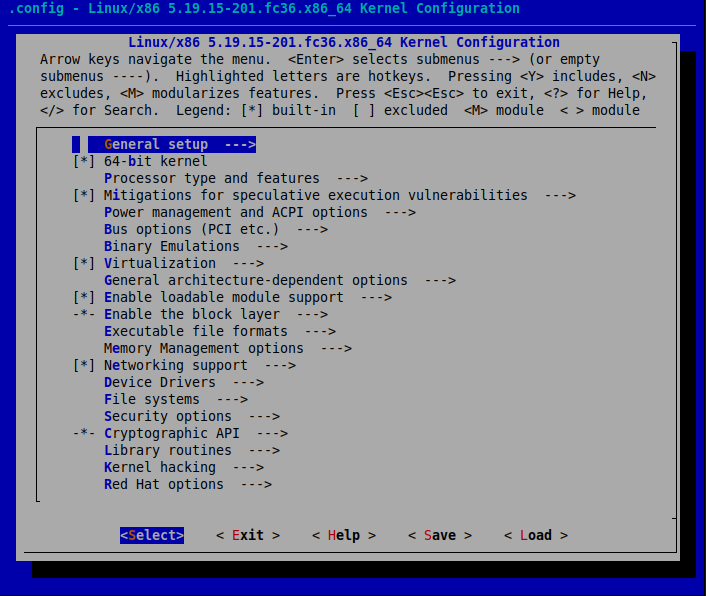
\includegraphics[width=0.8\linewidth]{1.png}}
\caption{начальное окно выбора модулей ядра}
\label{ris:nachalo}
\end{figure}

}

\end{document}
\end{verbatim}

\includepdf[landscape=true,scale=0.8,pages={1-3}]{Informatika_presentation}

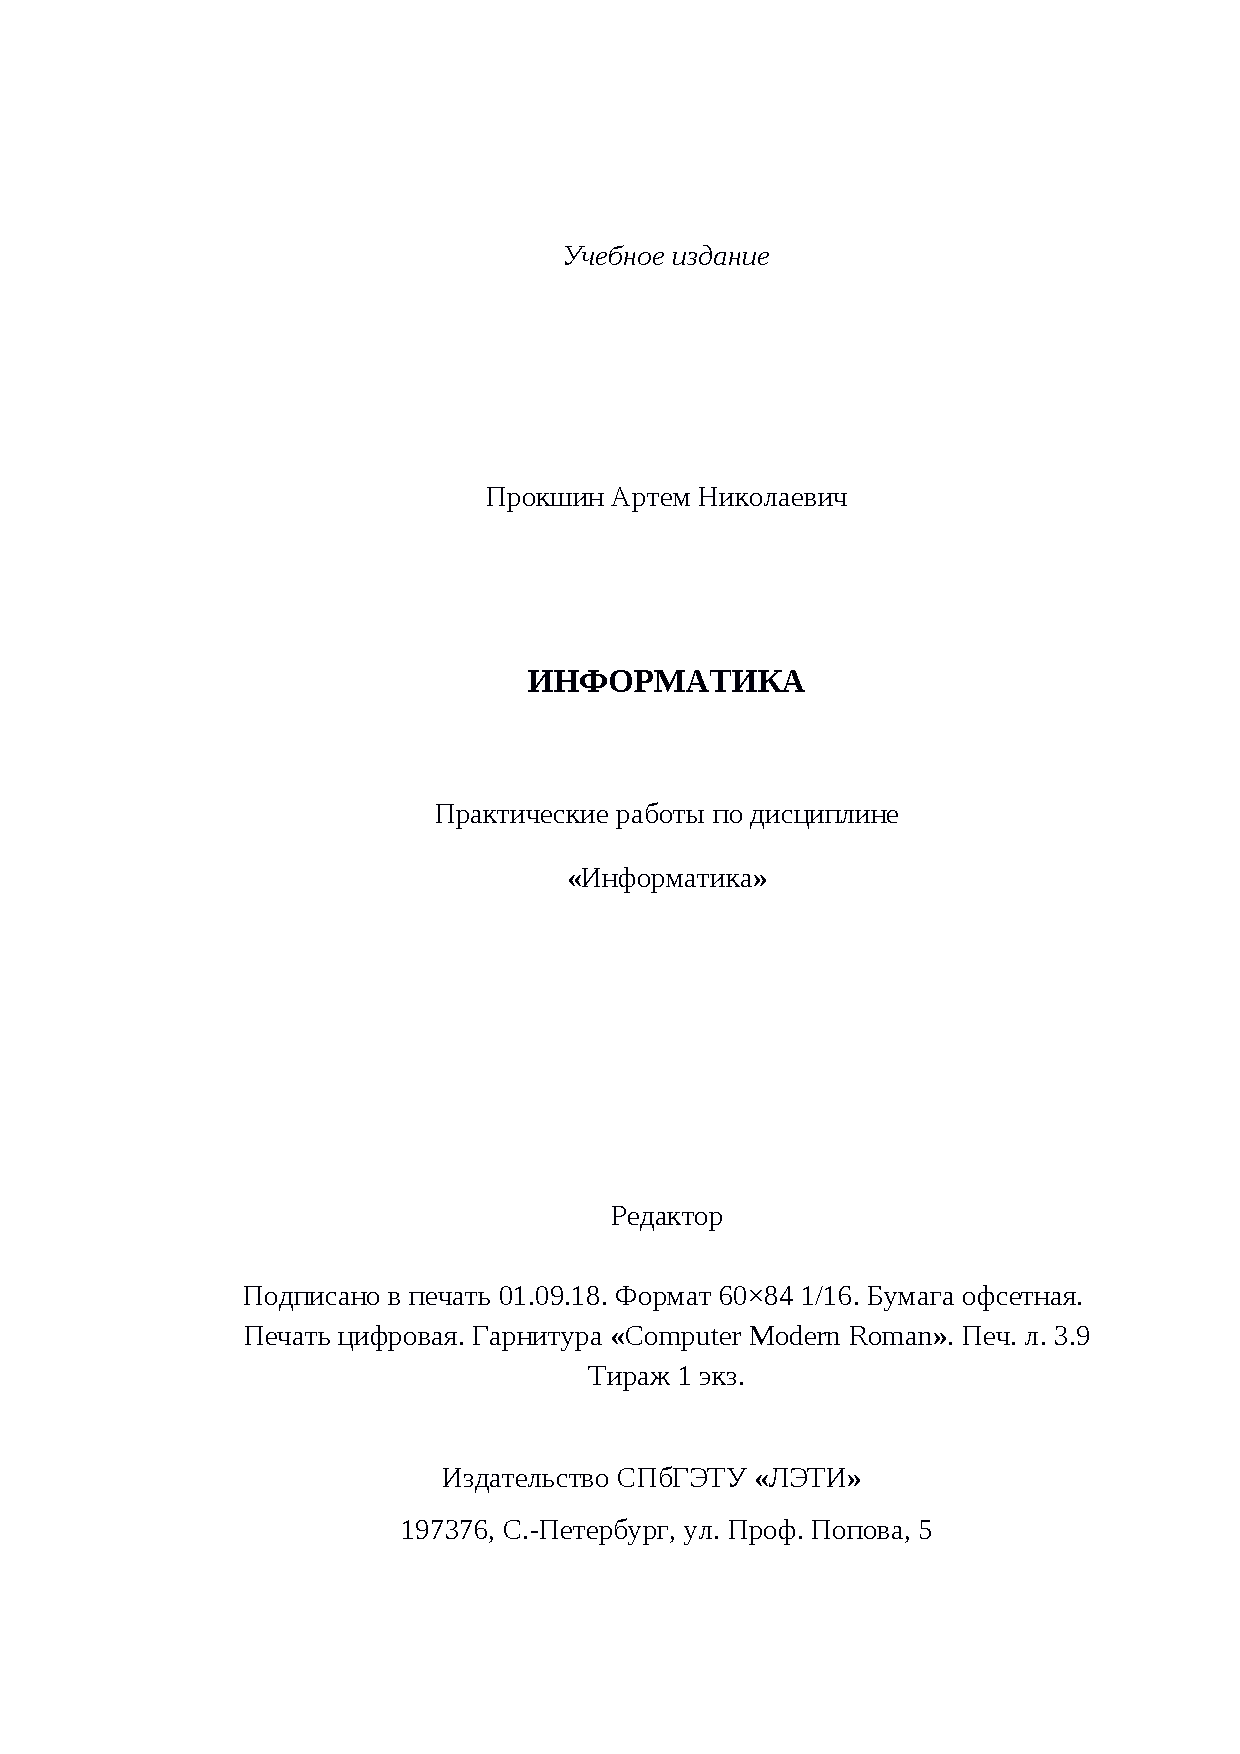
\includepdf[pages=-]{Informatika_praktika_last}
\end{document}
